%=====================================================================
%  Quantitative Reasoning - LAB 413
%  Lab 11: Z-tests, T-tests & Interaction Effects (Review Session)
%  Instructor: Subin Na
%  Beamer conversion of Lab11_1119_PPT.pptx
%  Compile: pdflatex Lab11_beamer.tex   (run twice for footline counters)
%=====================================================================
\documentclass[aspectratio=169,11pt]{beamer}

%---------------------------------------------------------------------
%  Packages
%---------------------------------------------------------------------
\usepackage[utf8]{inputenc}
\usepackage[T1]{fontenc}
\usepackage{lmodern}
\usepackage{amsmath,amssymb}
\usepackage{graphicx}
\usepackage{booktabs}
\usepackage{tcolorbox}
\tcbuselibrary{skins}

%---------------------------------------------------------------------
%  QR-Lab 413 theme  (shared across all 11 labs)
%---------------------------------------------------------------------
\usetheme{default}
\usecolortheme{default}
\useinnertheme{circles}

\definecolor{qrnavy}{RGB}{20,44,90}
\definecolor{qrblue}{RGB}{38,80,150}
\definecolor{qrgray}{RGB}{90,95,105}
\definecolor{qrlight}{RGB}{234,239,247}
\definecolor{qrred}{RGB}{190,60,60}

\setbeamercolor{structure}{fg=qrnavy}
\setbeamercolor{frametitle}{fg=white,bg=qrnavy}
\setbeamercolor{title}{fg=qrnavy}
\setbeamercolor{block title}{fg=white,bg=qrblue}
\setbeamercolor{block body}{bg=qrlight}
\setbeamercolor{itemize item}{fg=qrblue}
\setbeamercolor{itemize subitem}{fg=qrblue}
\setbeamerfont{frametitle}{series=\bfseries}
\setbeamertemplate{navigation symbols}{}

% Frametitle bar
\setbeamertemplate{frametitle}{%
  \nointerlineskip
  \begin{beamercolorbox}[wd=\paperwidth,ht=3.2ex,dp=1.2ex,leftskip=0.3cm]{frametitle}%
    \strut\insertframetitle\strut
  \end{beamercolorbox}%
}

% Footline: course | lab | slide number
\newcommand{\labnum}{Lab 11}
\setbeamertemplate{footline}{%
  \leavevmode%
  \hbox{%
    \begin{beamercolorbox}[wd=.5\paperwidth,ht=2.4ex,dp=1ex,leftskip=.3cm]{author in head/foot}%
      \usebeamerfont{author in head/foot}\color{qrgray}\small Quantitative Reasoning -- LAB 413%
    \end{beamercolorbox}%
    \begin{beamercolorbox}[wd=.5\paperwidth,ht=2.4ex,dp=1ex,rightskip=.3cm]{title in head/foot}%
      \usebeamerfont{title in head/foot}\color{qrgray}\small\hfill \labnum \quad\insertframenumber\,/\,\inserttotalframenumber%
    \end{beamercolorbox}}%
}

% Number badge (01, 02, ...) used on concept slides
\newtcbox{\numbadge}{on line,boxsep=2pt,left=4pt,right=4pt,top=2pt,bottom=2pt,
  colback=qrnavy,colframe=qrnavy,fontupper=\bfseries\color{white},arc=2pt}

% Key-concepts block
\newtcolorbox{keybox}[1][Key Concepts]{colback=qrlight,colframe=qrnavy,
  fonttitle=\bfseries,title={#1},coltitle=white,arc=2pt,left=4pt,right=4pt,
  top=3pt,bottom=3pt,boxrule=0.6pt}

%---------------------------------------------------------------------
%  Title data
%---------------------------------------------------------------------
\title{\bfseries Z-tests, T-tests \& Interaction Effects}
\subtitle{Review Session \textbullet\ Lab 11}
\author{Instructor: Subin Na}
\institute{Quantitative Reasoning -- LAB 413}
\date{November 19, 2025}

\begin{document}

%---------------------------------------------------------------------
%  Title slide
%---------------------------------------------------------------------
{\setbeamertemplate{footline}{}
\begin{frame}
  \vfill
  {\color{qrgray}\small Quantitative Reasoning -- LAB 413}\\[0.6em]
  {\usebeamerfont{title}\color{qrnavy}\huge\bfseries Z-tests, T-tests\\[0.15em]\& Interaction Effects\par}
  \vspace{0.4em}
  {\color{qrblue}\large Review Session \ \textbullet\ \ Lab 11}\par
  \vspace{1.6em}
  {\color{qrgray} Instructor: \textbf{Subin Na} \hfill November 19, 2025}
  \vfill
\end{frame}
}

%---------------------------------------------------------------------
%  Today's Plan
%---------------------------------------------------------------------
\begin{frame}{Today's Plan}
  \begin{columns}[T]
    \begin{column}{0.5\textwidth}
      \textbf{\color{qrnavy}1. Quick Review}
      \begin{itemize}
        \item Z-tests and T-tests
        \item Choosing between them
        \item Worked exercises
        \item Interaction effects in regression
      \end{itemize}
    \end{column}
    \begin{column}{0.5\textwidth}
      \phantom{\textbf{x}}
      \vspace{0.8em}
      \textbf{\color{qrnavy}2. RStudio Practice}
      \begin{itemize}
        \item Interaction effects
      \end{itemize}
    \end{column}
  \end{columns}
\end{frame}

%---------------------------------------------------------------------
%  01 What is a Z-test?  (RECREATE formula)
%---------------------------------------------------------------------
\begin{frame}{\numbadge{01}\ \ What is a Z-test?}
  \begin{keybox}
    A hypothesis test used to compare a \textbf{sample mean} to a
    \textbf{population mean} when:
    \begin{itemize}
      \item The population standard deviation ($\sigma$) is \textbf{known}.
      \item The sample size is large ($n > 30$).
    \end{itemize}
  \end{keybox}
  \vspace{0.6em}
  \begin{center}
    \textbf{\color{qrnavy}Formula}
    \begin{equation*}
      Z = \frac{\bar{X}-\mu_0}{\sigma/\sqrt{n}}
    \end{equation*}
  \end{center}
\end{frame}

%---------------------------------------------------------------------
%  02 What is a T-test?  (RECREATE formula)
%---------------------------------------------------------------------
\begin{frame}{\numbadge{02}\ \ What is a T-test?}
  \begin{keybox}
    A hypothesis test to compare a \textbf{sample mean} to a
    \textbf{population mean} when:
    \begin{itemize}
      \item The population standard deviation is \textbf{unknown}.
      \item You estimate $\sigma$ using the sample standard deviation ($s$).
    \end{itemize}
  \end{keybox}
  \vspace{0.4em}
  \begin{center}
    \textbf{\color{qrnavy}Formula}
    \begin{equation*}
      t = \frac{\bar{X}-\mu_0}{s/\sqrt{n}}
    \end{equation*}
  \end{center}
  \vspace{0.2em}
  \begin{center}
    {\small The $t$-distribution accounts for the additional uncertainty from
    estimating $\sigma$.}
  \end{center}
\end{frame}

%---------------------------------------------------------------------
%  Decision flowchart  (EMBED drawn diagram)
%---------------------------------------------------------------------
\begin{frame}{Choosing a Test: Z or T?}
  \begin{center}
    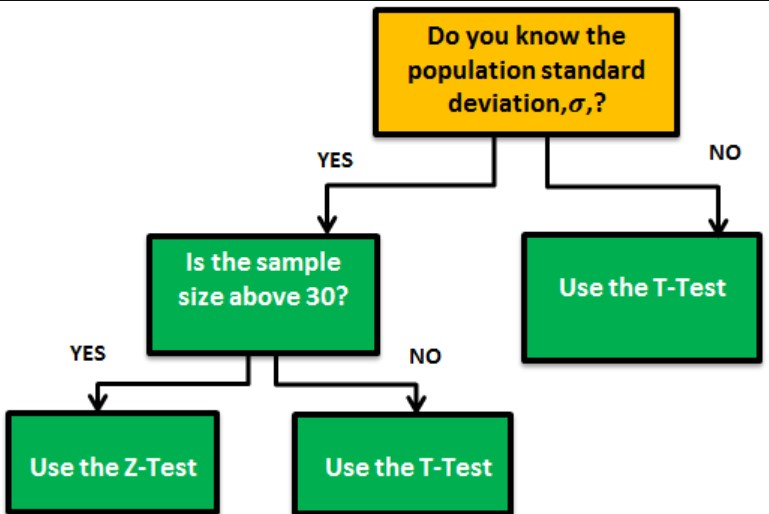
\includegraphics[height=0.78\textheight]{figures/s05_1_12.1x8.0.jpg}
  \end{center}
\end{frame}

%---------------------------------------------------------------------
%  03 Z-test vs. T-test comparison table  (RECREATE booktabs)
%---------------------------------------------------------------------
\begin{frame}{\numbadge{03}\ \ Z-test vs.\ T-test (Comparison)}
  \begin{center}
  \renewcommand{\arraystretch}{1.4}
  \begin{tabular}{@{}lll@{}}
    \toprule
    \textbf{Criterion} & \textbf{Z-test} & \textbf{T-test}\\
    \midrule
    Sample Size        & Typically large ($n > 30$) & Any size, especially $n \le 30$\\
    Population SD ($\sigma$) & Known                 & Unknown (use sample SD)\\
    Distribution       & Standard Normal            & $t$-distribution ($df = n-1$)\\
    Test Statistic     & $\sigma$ used              & $s$ used\\
    \bottomrule
  \end{tabular}
  \end{center}
\end{frame}

%---------------------------------------------------------------------
%  Exercise 1
%---------------------------------------------------------------------
\begin{frame}{Exercise 1}
  \begin{keybox}[Scenario]
    You have a sample of \textbf{50 people's weights}, and the population
    standard deviation is \textbf{known}. You want to test whether the sample
    comes from a population with mean $= 150$ lbs.
  \end{keybox}
  \vspace{0.8em}
  \begin{tcolorbox}[colback=qrlight,colframe=qrblue,arc=2pt,boxrule=0.6pt]
    \textbf{\color{qrnavy}Use a Z-test.}\\
    Reason: $\sigma$ known $+$ $n > 30$.
  \end{tcolorbox}
\end{frame}

%---------------------------------------------------------------------
%  Exercise 2
%---------------------------------------------------------------------
\begin{frame}{Exercise 2}
  \begin{keybox}[Scenario]
    A botanist studies a new soil additive advertised to promote faster plant
    growth. After applying it across greenhouse units, the botanist measures the
    final height of \textbf{300 plants} grown under the treatment. No prior study
    provides a reliable estimate of the population standard deviation for this
    species. The botanist wants to evaluate whether the average plant height
    differs from the manufacturer's claim of \textbf{20 cm}.
  \end{keybox}
  \vspace{0.5em}
  \begin{tcolorbox}[colback=qrlight,colframe=qrblue,arc=2pt,boxrule=0.6pt]
    \textbf{\color{qrnavy}Use a T-test.}\\
    Reason: $\sigma$ unknown (the sample SD must be used).
  \end{tcolorbox}
\end{frame}

%---------------------------------------------------------------------
%  Exercise 3
%---------------------------------------------------------------------
\begin{frame}{Exercise 3}
  \begin{keybox}[Scenario]
    A large hospital system evaluates whether a newly implemented treatment
    protocol affects average recovery time. Clinical records from past years
    provide a reliable estimate of the population standard deviation. A research
    team collects data on \textbf{200 patients} who received the updated
    treatment and records their recovery times, to examine whether the new
    protocol leads to a \emph{different} average recovery time than the standard
    approach.
  \end{keybox}
  \vspace{0.4em}
  \begin{tcolorbox}[colback=qrlight,colframe=qrblue,arc=2pt,boxrule=0.6pt]
    \textbf{\color{qrnavy}Use a Z-test.}\\
    Reason: $\sigma$ known $+$ large sample.
  \end{tcolorbox}
\end{frame}

%---------------------------------------------------------------------
%  04 Interaction Effects in Regression
%---------------------------------------------------------------------
\begin{frame}{\numbadge{04}\ \ Interaction Effects in Regression}
  \begin{keybox}
    An \textbf{interaction effect} means the effect of one predictor on the
    outcome \emph{depends on} the value of another predictor.
  \end{keybox}
  \vspace{0.6em}
  \textbf{\color{qrnavy}In R, the \texttt{*} operator expands to main effects
  plus the interaction:}
  \begin{equation*}
    \texttt{x1 * x2} \;=\; \texttt{x1} \;+\; \texttt{x2} \;+\; \texttt{x1:x2}
  \end{equation*}
  \vspace{0.2em}
  \begin{itemize}
    \item The \texttt{x1:x2} term captures how the slope of one variable
          \emph{shifts} across levels of the other.
  \end{itemize}
\end{frame}

%---------------------------------------------------------------------
%  05 Binary x Continuous Interaction
%---------------------------------------------------------------------
\begin{frame}{\numbadge{05}\ \ Binary $\times$ Continuous Interaction}
  \begin{keybox}
    When a \textbf{binary} variable interacts with a \textbf{continuous} one,
    each group gets its \emph{own slope} for the continuous predictor.
  \end{keybox}
  \vspace{0.5em}
  \begin{equation*}
    Y = \beta_0 + \beta_1 D + \beta_2 X + \beta_3 (D \times X) + \varepsilon
  \end{equation*}
  \begin{itemize}
    \item When $D = 0$: \quad slope of $X$ is $\beta_2$.
    \item When $D = 1$: \quad slope of $X$ is $\beta_2 + \beta_3$.
    \item $\beta_3$ is the \textbf{difference in slopes} between the two groups.
  \end{itemize}
\end{frame}

%---------------------------------------------------------------------
%  Transition to RStudio
%---------------------------------------------------------------------
{\setbeamertemplate{footline}{}
\begin{frame}
  \vfill
  \centering
  {\color{qrnavy}\Huge\bfseries RStudio Practice}\\[0.8em]
  {\color{qrblue}\large Regression with Interaction Terms}\\[0.4em]
  {\color{qrgray} See \texttt{Lab11.Rmd} / \texttt{Lab11\_1119.R}}
  \vfill
\end{frame}
}

\end{document}
